\documentclass[pdf]{beamer}
\usepackage{multicol}
\mode<presentation>{}
\usetheme{Warsaw}
\usepackage{subcaption}
%\usepackage{listings}

\title{Clustering por ES, EP e variantes}
\author{Gabriel Evangelista}
\begin{document}

\begin{frame}{Proposta e Resultados Parciais}
	\begin{columns}
		\column{.6\linewidth}
		Algoritmos:
		\begin{itemize}
			\item Evolution Strategies (ES) 
%			\item ES - Controle de Parâmetros - Regra de Rechenberg
			\item ES - Multimodal - Ilhas constantes
			\item ES - Memético - Potêncial GLA
			\item Evolutionary Programming (EP)
			\item EP - Distribuição de Cauchy (FEP)
		\end{itemize}
	
	
		Características comuns:
		\begin{itemize}
			\item Mutação: Não correlacionada de passo múltiplo ($ \varepsilon_0 = 10^{-3} $)
			\item Recombinação: X discreto e $ \sigma $ linear (ES/Variantes)
			\item Seleção de Sobreviventes:
			\begin{itemize}
				\item ES/Variantes: Elitismo ($ \mu, \lambda $)
				\item EP/Variantes: SUS ($ \mu + \lambda $)
			\end{itemize}
		\end{itemize}


		\column{.55\linewidth}
			\begin{figure}
				\begin{subfigure}[t]{0.55\textwidth}
					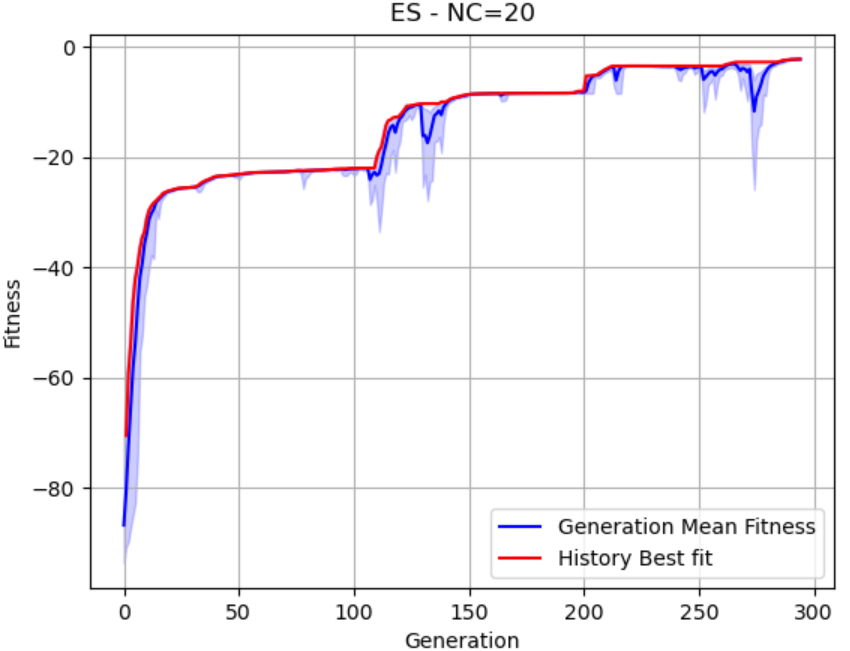
\includegraphics[width=\linewidth]{img/ES_NC20_exemplo.png}
				\end{subfigure}
				\begin{subfigure}[t]{0.55\textwidth}
					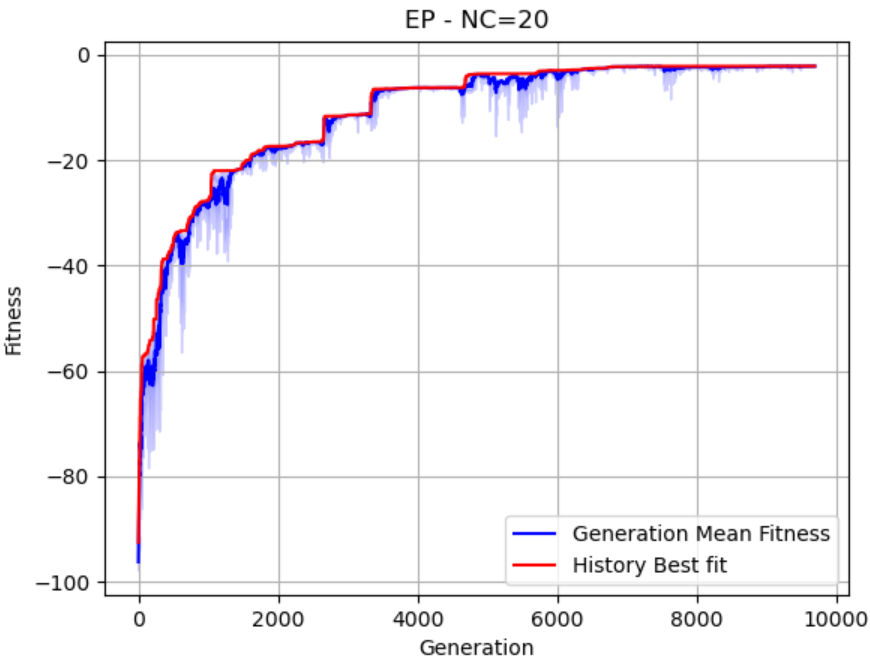
\includegraphics[width=\linewidth]{img/EP_NC20_exemplo.png}
				\end{subfigure}
				\begin{subfigure}[t]{0.55\textwidth}
					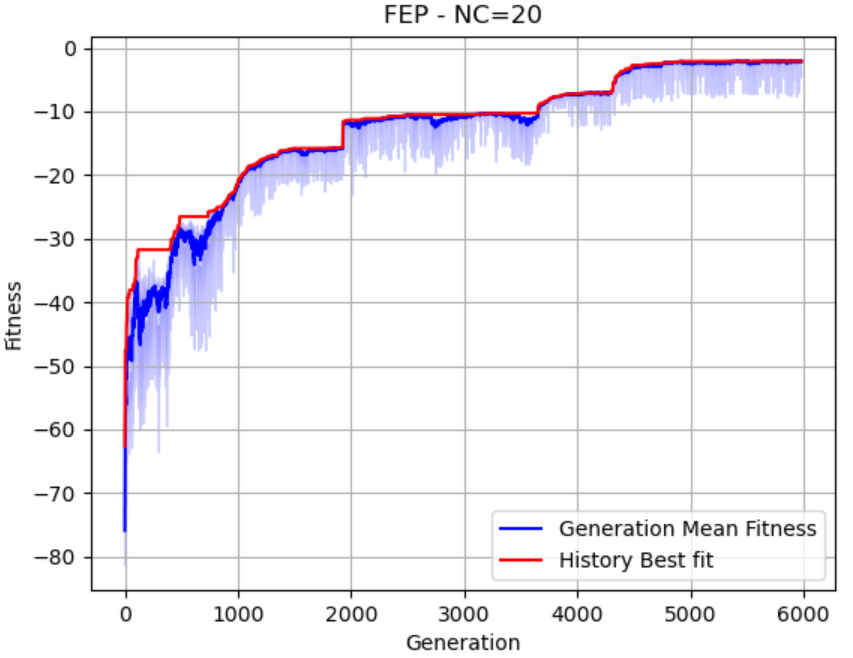
\includegraphics[width=\linewidth]{img/FEP_NC20_exemplo.png}
				\end{subfigure}
			\end{figure}
		
	\end{columns}
\end{frame}


\begin{frame}{Metodologia}
%	\begin{columns}
%		\column{\linewidth}
			\begin{itemize}
				\item Parâmetros variados comuns:
				\begin{itemize}
					\item $ \mu \in \{10, 30, 80\} $ 
					\item $ \lambda/\mu \in \{3, 7, 10, 25\} $
				\end{itemize}
				
				\item Limite computacional: $ 5\cdot 10^5 $ avaliações da função custo
				\item Dificuldade crescente: Número de Clusters ($ \mathbb{R}^2 $) $ \in \{10, 20, 30, ... \} $
				\item 35 lançamentos por configuração
				\item Sucesso: tolerância de $5\% \cdot J_{min} $
				\item Critérios: \textit{\textbf{SR}}, \textbf{MBF} e \textit{\textbf{AES}} dos melhores parâmetros em \textit{\textbf{SR}} 

			\end{itemize}
%	\end{columns}		
	\begin{columns}
		\column{.33\linewidth}
			\begin{block}{Multimodal}
			\begin{itemize}
				\item Ilhas / Especiação
				\item População $ C^{\underline{TE}}  $
				\item Parâmetros: 
				\begin{itemize}
					\item N ilhas
					\item T migração
					\item n imigrantes
				\end{itemize}
			\end{itemize}
			\end{block}
		
		\column{.33\linewidth}
		\begin{block}{Memético}
			\begin{itemize}
				\item \textit{Lamarck} (?)
				\item GLA $ \rightarrow $ Potencial
				\item Parâmetros:
				\begin{itemize}
					\item época
					\item n passos
				\end{itemize}
			\end{itemize}
			
		\end{block}
		\column{.33\linewidth}
		\begin{block}{Fast EP}
			$ \sigma' = \sigma \cdot e^{\tau_1 \cdot \mathcal{N} + \tau_2 \cdot \mathcal{N}_i} $
			$$ x_i' = x_i + \sigma' \cdot \mathcal{N}(0, 1) $$
			$$\downarrow$$
			$$ x_i' = x_i + \sigma' \cdot \mathcal{C}(0, 1) $$ 
		\end{block}
	\end{columns}



\end{frame}


\begin{frame}{Dúvidas}
	\begin{itemize}
		\item É esperado bom resultado do algoritmo memético proposto?
		\item Controle de parâmetro, vale a pena a comparação? Usar ou não o controle do $ \sigma $ pelo Regra de Rechemberg nas demais variantes?
		\item Vale a pena variar $ \tau_1 $ e $ \tau_2 $ ?
		\item É válido Controlar a dispersão da população inicial? Conta como modificação?
	\end{itemize}
\end{frame}

\end{document}
